%------------------------------------------------
% LaTex File created by Miguel A. Torres-Torriti
% 2008.03.22
% REF: Assingments/Tests/
% REF: Function References and Manual.
%      Added on 2011.03.27 based on the 
%      Lie Tools Package user's guide.
%------------------------------------------------
%1in=25.4mm=72.27pt
%1pc=12pt (pc Pica, pt Point)
%1pt=0.35mm
%Matlab figure ratio X/Y = 1.28
%
\documentclass[11pt,letterpaper,twoside]{report}%{article}
\def\doctitle{Plantilla \LaTeX para Informes} % Título/Tema de la Sección
\def\docsubtitle{} % Nombre del curso
\def\docdate{2015.05.28} % Fecha del documento
\def\coursename{IRB2002 -- Diseño de Sistemas Robóticos} % Sigla -- Nombre del Curso
\def\authorname{Miguel Torres} % Su nombre y apellido 
\def\deptname{Escuela de Ingenier\'ia} % El nombre de su Escuela/Unidad Académica
\def\orgname{Pontificia Universidad Cat\'olica de Chile} % Nombre de la Universidad

%--------- LOAD PACKAGES ---------
%--- template and layout ---
\usepackage{fancyhdr}
%\usepackage{makeidx}
\usepackage{float}
\usepackage{multirow}
\usepackage[utf8]{inputenc}

%--- algorithms ---
\usepackage[spanish]{algorithm2e}
%\usepackage{algorithm}     used together with 'algorithmic' for IEEE pseudocode style
%\usepackage{algorithmic}   used together with 'algorithm' for IEEE pseudocode style

% --- other special packages ---
%\usepackage{cancel} % to write cancel signs on mathematical expressions 
%\renewcommand{\CancelColor}{\red}
%\usepackage{moreverb} % special verbatim formatting. keeps tabs
 
%--- graphics, colors and drawings ---
\usepackage{graphicx}
%\usepackage{epsfig}
%\usepackage[hang]{caption}
%\usepackage{graphics}   %Has trouble positioning/rescaling postscripts.
\usepackage[svgnames]{xcolor} %required by xfig combined ps/tex figures.
                     %required by \definecolor{newcolorname}{named}{somecolor}
										 % The 'color' package does not support definecolor.

%- color definitions -
\usepackage{ifthen} % required by the colordefs
% Booleans for color palette definition
\newboolean{narcel}
\newboolean{amaazu}
\newboolean{negdor}
\newboolean{celbla}
\newboolean{celro}
\newboolean{rocel}
\newboolean{azubla}
\newboolean{planeg}
\newboolean{celneg}
\newboolean{grineg}
\newboolean{blaneg}
\newboolean{negbla}
\newboolean{taller2011}
\newboolean{celazu}
\newboolean{UCflama}
\newboolean{mono}

\setboolean{amaazu}{true}


% Color definitions - Pantone Coated (CVC) / Pantone Metallics Varnished (CVV)


\definecolor{UC185}{rgb}{0.9922,0.0941,0.1647}    % {253,24,42}    rojo: Pantone 185 CVC
\definecolor{UC136}{rgb}{1.0000,0.7255,0.2118}   % {255,185,54}   amarillo: Pantone 136 CVC
\definecolor{UC2707}{rgb}{0.7333,0.8275,0.9059} % {187,211,231} celeste claro: Pantone 2707 CVC
\definecolor{UC2718}{rgb}{0.3137,0.4627,0.7137} %{80,118,182} celeste: Pantone 2718 CVC
\definecolor{UC2727}{rgb}{0.1529,0.3294,0.8275}  % {39,84,211} azul celeste: Pantone 2727 CVC
\definecolor{UC2728}{rgb}{0.0863,0.1882,0.6510}   % {22,48,166}  azul: Pantone 2728 CVC
\definecolor{UC871}{rgb}{0.5882,0.4706,0.2588}   % {150,120,66}  dorado: Pantone 871 CVV
\definecolor{UC877}{rgb}{0.4863,0.5137,0.5255}  % {124,131,134}  plateado: Pantone 877 CVV

\definecolor{nar01}{rgb}{0.8667,0.5020,0.2784}  % {} naranjo office
\definecolor{cel01}{rgb}{0.5804,0.7137,0.8235}  % {148,182,210) celeste office
\definecolor{caf01}{rgb}{0.4667,0.3725,0.3333}  % {119,95,85) cafe office

\definecolor{azu01}{rgb}{0.4471,0.4863,0.6392}  % {} azul morado
\definecolor{ver01}{rgb}{0.8236,0.8549,0.4784}  % {148,182,210) verde amarillo
\definecolor{azu02}{rgb}{0.6235,0.7216,0.8039}  % {119,95,85) azul claro

% amarillo azul UC136 UC2728
\ifthenelse{\boolean{amaazu}}{%
\definecolor{colorlargeA}{named}{UC136} 
\definecolor{colorshortA}{named}{UC2728}
\definecolor{colorlargeB}{named}{UC136} 
\definecolor{colorshortB}{named}{UC2728}
}{}

% negro dorado black UC871
\ifthenelse{\boolean{negdor}}{
\definecolor{colorlargeA}{named}{black} 
\definecolor{colorshortA}{named}{UC871}
\definecolor{colorlargeB}{named}{black} 
\definecolor{colorshortB}{named}{UC871}
}{}

% azul-celeste blanco UC2727 white
\ifthenelse{\boolean{celbla}}{
\definecolor{colorlargeA}{named}{UC2727} 
\definecolor{colorshortA}{named}{white}
\definecolor{colorlargeB}{named}{UC2727} 
\definecolor{colorshortB}{named}{white}
}{}


% azul-celeste rojo
\ifthenelse{\boolean{celro}}{
\definecolor{colorlargeA}{named}{UC2727} % celeste 
\definecolor{colorshortA}{named}{UC185}
\definecolor{colorlargeB}{named}{UC2727} % celeste  
\definecolor{colorshortB}{named}{UC185}
}{}

% rojo azul-celeste 
\ifthenelse{\boolean{rocel}}{
\definecolor{colorshortA}{named}{UC2727} % celeste 
\definecolor{colorlargeA}{named}{UC185}
\definecolor{colorshortB}{named}{UC2727} % celeste  
\definecolor{colorlargeB}{named}{UC185}
}{}

% azul blanco UC2728 white
\ifthenelse{\boolean{azubla}}{
\definecolor{colorlargeA}{named}{UC2728} 
\definecolor{colorshortA}{named}{white}
\definecolor{colorlargeB}{named}{UC2728} 
\definecolor{colorshortB}{named}{white}
}{}

% blanco azul white UC2728
\ifthenelse{\boolean{planeg}}{
\definecolor{colorshortA}{named}{UC877} 
\definecolor{colorlargeA}{named}{black}
\definecolor{colorshortB}{named}{UC877} 
\definecolor{colorlargeB}{named}{black}
}{}


% negro celeste black UC2707
\ifthenelse{\boolean{celneg}}{
\definecolor{colorlargeA}{named}{black} 
\definecolor{colorshortA}{named}{UC2707}
\definecolor{colorlargeB}{named}{black} 
\definecolor{colorshortB}{named}{UC2707}
}{}

% gris negro gray black 
\ifthenelse{\boolean{grineg}}{
\definecolor{colorlargeA}{named}{black} 
\definecolor{colorshortA}{gray}{0.8}
\definecolor{colorlargeB}{named}{black} 
\definecolor{colorshortB}{gray}{0.8}
}{}

% blanco negro white black 
\ifthenelse{\boolean{blaneg}}{
\definecolor{colorlargeA}{named}{black} 
\definecolor{colorshortA}{named}{white}
\definecolor{colorlargeB}{named}{black} 
\definecolor{colorshortB}{named}{white}
}{}

% negro blanco black white 
\ifthenelse{\boolean{negbla}}{
\definecolor{colorlargeA}{named}{white} 
\definecolor{colorshortA}{named}{black}
\definecolor{colorlargeB}{named}{white} 
\definecolor{colorshortB}{named}{black}
}{}

% Office 1
\ifthenelse{\boolean{narcel}}{
\definecolor{colorlargeA}{named}{cel01} 
\definecolor{colorshortA}{named}{nar01}
\definecolor{colorlargeB}{named}{cel01} 
\definecolor{colorshortB}{named}{nar01}
}{}

% Taller 2011
\ifthenelse{\boolean{taller2011}}{
\definecolor{colorlargeA}{named}{azu01} 
\definecolor{colorshortA}{named}{ver01}
\definecolor{colorlargeB}{named}{azu01} 
\definecolor{colorshortB}{named}{ver01}
}{}

% celeste azul UC2707 UC2728
\ifthenelse{\boolean{celazu}}{
\definecolor{colorlargeA}{named}{UC2728} % texto izq.
\definecolor{colorshortA}{named}{UC2707} % fondo izq.
\definecolor{colorlargeB}{named}{UC2728} % fondo der.
\definecolor{colorshortB}{named}{UC2707}  % texto der.
}{}

% izq (bgnd,fgnd): amarillo azul, der (bgnd,fgnd): plateado/gris amarillo  UC136 UC2728 UC877 UC136
\ifthenelse{\boolean{UCflama}}{
\definecolor{colorlargeA}{named}{UC2728} % texto izq.
\definecolor{colorshortA}{named}{UC136} % fondo izq.
\definecolor{colorlargeB}{named}{UC877} % fondo der.
\definecolor{colorshortB}{named}{UC136}  % texto der.
}{}

% Mono 
\ifthenelse{\boolean{mono}}{
\definecolor{colorlargeA}{named}{colorlargeA} 
\definecolor{colorshortA}{named}{colorshortA}
\definecolor{colorlargeB}{named}{colorshortA} 
\definecolor{colorshortB}{named}{colorlargeA}
}{
% \definecolor{colorlarge} {named}{colorlargeA}
% \definecolor{colorshort}{named}{colorshortA}
% \definecolor{colorlargeB}{named}{colorlarge} 
% \definecolor{colorshortB}{named}{colorshort}
}
 \definecolor{colorlarge}{named}{colorlargeA}
 \definecolor{colorshort}{named}{colorshortA}



\definecolor{colordatehead}{named}{colorlarge} 
\definecolor{colorseclab}{named}{colorshort} 
\definecolor{colorchapter}{named}{colorshort}

\definecolor{navy}{rgb}{0.1,0.2,0.5}

%\usepackage{dictsym}
\usepackage{manfnt}  %\manimpossiblecube
\usepackage{dingbat} %\smallpencil \leftpointright
%\usepackage[alpine,clock,electronic,geometry,misc,weather]{ifsym} % \Radiation

%\usepackage{stix}
%%http://tex.stackexchange.com/questions/174814/how-to-get-only-one-symbol-from-a-symbol-package
%\DeclareFontFamily{U}{stixextrai}{}
%\DeclareFontShape{U}{stixextrai}{m}{n}
 %{ <-> stix-extra1 }{}
%
%\newcommand{\WolframSym}{{\usefont{U}{stixextrai}{m}{n}\symbol{132}}}
%%http://blog.wolframalpha.com/2009/05/19/whats-in-the-logo-that-which-we-call-a-rhombic-hexecontahedron/
% %Put in text: \WolframSym
%https://en.wikipedia.org/wiki/List_of_uniform_polyhedra

%\usepackage{uni}
   %\renewcommand{\bausquare}{{\usefont{OT1}{uni}{m}{n}\char"00}}
   %\renewcommand{\baucircle}{{\usefont{OT1}{uni}{m}{n}\char"01}}
   %\renewcommand{\bautriangle}{{\usefont{OT1}{uni}{m}{n}\char"02}}
   %\renewcommand{\bauhead}{{\usefont{OT1}{uni}{m}{n}\char"03}}
   %\renewcommand{\bauforms}{{\usefont{OT1}{uni}{m}{n}\char"04}}

%\usepackage{universal}	
%   \newcommand{\bauface}{{\usefont{OT1}{universal}{m}{n}\char"10}}
%


%--- fonts ---
%\usepackage{amsfonts}
% A popular package from the American Mathematical Society that provides
% many useful and powerful commands for dealing with mathematics. If using
% it, be sure to load this package with the cmex10 option to ensure that
% only type 1 fonts will utilized at all point sizes. Without this option,
% it is possible that some math symbols, particularly those within
% footnotes, will be rendered in bitmap form which will result in a
% document that can not be IEEE Xplore compliant!
%
% Also, note that the amsmath package sets \interdisplaylinepenalty to 10000
% thus preventing page breaks from occurring within multiline equations. Use:
%\interdisplaylinepenalty=2500
% after loading amsmath to restore such page breaks as IEEEtran.cls normally
% does. amsmath.sty is already installed on most LaTeX systems. The latest
% version and documentation can be obtained at:
% http://www.ctan.org/tex-archive/macros/latex/required/amslatex/math/
\usepackage{amsfonts}
\usepackage{amssymb}
\usepackage[cmex10]{amsmath}
%These Packages are obsolete.
%\usepackage{amstex}
%\usepackage{latexsym}

\usepackage{bm} % included for bold greek fonts, see: http://tex.stackexchange.com/questions/595/how-can-i-get-bold-math-symbols

%% --- IEEE Times Configuration ---
%% IEEE uses Times Roman font, so we'll default to Times.
%% These three commands make up the entire times.sty package.
%\renewcommand{\sfdefault}{phv} % Postscript Helvetica (Adobe)
%\renewcommand{\rmdefault}{ptm} % Postscript Times Modern (Adobe)
%\renewcommand{\ttdefault}{pcr} % Postscript Courier (Adobe)
%
%
%%\@IEEEcompsoconly{\typeout{-- Using IEEE Computer Society mode.}}
%
%% V1.7 compsoc nonconference papers, use Palatino/Palladio as the main text font,
%% not Times Roman.
%%\@IEEEcompsocnotconfonly{\renewcommand{\rmdefault}{ppl}}
%
%% enable Times/Palatino main text font
%\normalfont\selectfont
%% --- end of IEEE Times Configuration

% --- Package Helvetica ---
%\usepackage{helvet}

% --- Package Sans ---
% Computer Modern Sans Serif
%https://www.ctan.org/pkg/sans
\usepackage{sans}
\renewcommand{\rmdefault}{cmss}
\renewcommand{\sfdefault}{cmr}

%\normalfont\selectfont

% --- Other Fonts ---
%http://en.wikibooks.org/wiki/LaTeX/Fonts
%\renewcommand{\rmdefault}{ppl} % Palatino
%\renewcommand{\rmdefault}{iwona} % Iwona

%\renewcommand{\rmdefault}{lmss} % Latin Modern Sans Serif

% --- Own configuration ---
%\renewcommand{\sfdefault}{ptm} % Times Modern
%\renewcommand{\rmdefault}{lmss} % Latin Modern Sans Serif
%\renewcommand{\ttdefault}{pcr} % Courier

\usepackage{iwona} % changes only text to Iwona
%\usepackage[math]{iwona} % changes text and math to Iwona
\usepackage[T1]{fontenc}

%\usepackage{kurier} % changes only text to Iwona
%\usepackage[math]{kurier} % changes text and math to Iwona
%\usepackage[T1]{fontenc}

%\usepackage{sans}
%\usepackage[T1]{fontenc} % MUST be loaded toghether with {sans} package, otherwise
                          % bold italic sans serif fonts appear as regular bold sans serif font.


%\usepackage{sans}
%\usepackage[T1]{fontenc} % MUST be loaded toghether with {sans} package, otherwise
                          % bold italic sans serif fonts appear as regular bold sans serif font.
%\renewcommand{\rmdefault}{phv}

%\DeclareMathAlphabet{\mathbfit}{OML}{cmm}{b}{it}

\usepackage[latin1]{inputenc} % must save as ANSI (not UTF-8) for this package to 
                               % work directly with characters that have an accent.


% --- Special boxes ---
% Must go after the fonts to avoid options clash between tcolorbox and amsmath.
\usepackage[skins,theorems]{tcolorbox}

\newtcolorbox{defbox}[1]{skin=widget,colback=blue!15!white,
colframe=blue!45!black,fonttitle=\bfseries,
title=\large\rule{0mm}{\baselineskip}\smallpencil~#1}

%\newtcolorbox[auto counter,number within=section, number freestyle={\noexpand\thechapter.\noexpand\thesection\noexpand\arabic{\tcbcounter}}]{
\newtcolorbox[auto counter,number within=section, number freestyle={\noexpand\thesection\noexpand\arabic{\tcbcounter}}]{exbox}[1]{colback=green!15!white,
colframe=green!45!black,fonttitle=\bfseries,
title={\LARGE\manimpossiblecube}\large~Ejemplo~\thetcbcounter #1}

\newtcolorbox{tipbox}[2][]{colback=red!5!white,
colframe=red!75!black,fonttitle=\bfseries,
colbacktitle=red!85!black,enhanced,
attach boxed title to top left={yshift=-2mm},
title={\LARGE \leftpointright} \large Debes saber que\ldots#2,#1}

\newcommand{\eqbox}[1]{\tcboxmath[enhanced,colback=yellow!50!white,colframe=red!60!black,arc=4pt,boxrule=1pt,drop fuzzy shadow]{ #1 }}


%hyperref package - Must be loaded at the end.
\usepackage{hyperref}
\hypersetup{
%    bookmarks=true,         % show bookmarks bar?
%    unicode=false,          % non-Latin characters in Acrobat's bookmarks
%    pdftoolbar=true,        % show Acrobat's toolbar?
%    pdfmenubar=true,        % show Acrobat's menu?
    pdffitwindow=false,     % window fit to page when opened
    pdfstartview={FitH},    % fits the width of the page to the window
%    pdftitle={My title},    % title
%    pdfauthor={Author},     % author
%    pdfsubject={Subject},   % subject of the document
%    pdfcreator={Creator},   % creator of the document
%    pdfproducer={Producer}, % producer of the document
%    pdfkeywords={keyword1} {key2} {key3}, % list of keywords
    pdfnewwindow=true,      % links in new window
    colorlinks=true,       % false: boxed links; true: colored links
    linkcolor=red,          % color of internal links
    citecolor=green,        % color of links to bibliography
    filecolor=magenta,      % color of file links
    urlcolor=cyan           % color of external links
}

\usepackage{pdfpages} % para incluir pdfs
%\includepdf[pages={1-2},landscape=false]{Instrucciones_Armado.pdf}
%\includepdf[pages={1},landscape=false]{legs_2_dof.pdf}

%\usepackage[novbox]{pdfsync} % Do not use pdfsync without [novbox], because it changes the layout of the description table of the LegoUC template!!!  MTT.2012.05.31... the problem was fixed with the [novbox] option
% pdfsync bugs
% ------------
% pdfsync uses extremely severe code. You should not use pdfsync on final documents because it can change the layout rather significantly
% (different page/line breaks are the most obvious changes), despite this is rather rare,
% 17.8th Murphy's law states that it will happen to you when it absolutely must not...

\usepackage{fancyvrb}


%--------- SET DIMENSIONS ---------
%DEFAULT SIZE: [letterpaper = 8.5in x 11in = 216mm x 279mm]
\topmargin -25.4mm %-15.4mm
\headheight 25mm %12mm
\headsep .5\baselineskip
\textheight 229mm %239mm
\footskip 1.5\baselineskip %3.5mm
%\footheight 0mm
\oddsidemargin 4.6mm %-5.4mm
\evensidemargin 4.6mm %-5.4mm
\textwidth 156mm %176mm
%\columnsep 0.375in

\parindent 0mm
\parskip 10pt
%\bibindent XXmm
\renewcommand{\baselinestretch}{1.0} %sets line spacing.


%--------- PAGE STYLE SETTINGS ---------
%\pagestyle{fancyplain} %forces fancy even on first chapter pages
\pagestyle{fancy}
\renewcommand{\headrulewidth}{0.4pt}
\renewcommand{\footrulewidth}{0.4pt}

%\fancyhead{} % clear all header fields
%\fancyhead[RO,LE]{\bfseries The performance of new graduates}
%\fancyfoot{} % clear all footer fields
%\fancyfoot[LE,RO]{\thepage}
%\fancyfoot[LO,CE]{From: K. Grant}
%\fancyfoot[CO,RE]{To: Dean A. Smith}

\lhead{% 
 %color{UC2707}
  {\large \coursename}\\
%  \deptname\\
  {\footnotesize \sc \orgname}}
\chead{}
\rhead{\parbox[b]{0.4\textwidth}{\raggedleft \Large \bf \color{UC2728}\doctitle}\!\!%
\setlength{\unitlength}{1mm}
\begin{picture}(0,0)
%\put(2.3,-41){\color{UC2728}\rule[0mm]{29mm}{.2mm}}
\put(3,-36){
\includegraphics[scale=0.47]{figs/logo_uc.pdf}}
\put(2.3,-1.58){\color{UC2728}\rule[0mm]{29mm}{27mm}}
%\put(2.3,-41){\color{UC2728}\rule[0mm]{0.2mm}{42.4mm}}
%%\put(30.6,-41){\color{UC2728}\rule[0mm]{0.2mm}{42.4mm}}
\end{picture}
}
\lfoot{\mbox{}\color{UC2728}\raisebox{.1\baselineskip}{\copyright}\ \deptname\ -\ \authorname.} %, \textrm{\docdate}}
\cfoot{}
\rfoot{\mbox{}\color{UC2728}\textrm{\thepage}}

% Redefine plain pagestyle used in the first page of each chapter
\fancypagestyle{plain}{%
%\fancyhf{} % clear all header and footer fields
\fancyhead[R]{}
\fancyfoot[R]{\mbox{}\color{UC2728}\thepage} % except the center
\renewcommand{\headrulewidth}{0.4pt}
\renewcommand{\footrulewidth}{0.4pt}}
%\renewcommand{\thesection}{\textsf{\arabic{section}}.}
%\renewcommand{\thesubsection}{\textsf{\arabic{section}.\arabic{subsection}.}}
%\renewcommand{\thefigure}{\textsf{\arabic{figure}}}
\renewcommand{\thesection}{\arabic{section}.}
\renewcommand{\thesubsection}{\arabic{section}.\arabic{subsection}.}
%\renewcommand{\thesubsubsection}{\arabic{section}.\arabic{subsection}.\arabic{subsubsection}.}

%\setcounter{secnumdepth}{3} %to number sections, subsections and subsubsections
%\setcounter{tocdepth}{3}    %to include subsubsections in the table of contents

%--------- RENEWED COMMANDS --------
% Renew equation numbering to produce eq 3.1, 3.2, etc.
%\renewcommand{\theequation}{\arabic{section}.\arabic{equation}}

%--------- NEW COMMANDS ---------
% *** Environments ***
\newcommand{\benum}{\begin{enumerate}}
\newcommand{\eenum}{\end{enumerate}}
\newcommand{\bi}{\begin{itemize}}
\newcommand{\ei}{\end{itemize}}
\newcommand{\ba}{\begin{array}}
\newcommand{\ea}{\end{array}}
%\newcommand{\be}{\begin{equation}}
%\newcommand{\ee}{\end{equation}}
\newcommand{\eq}[1]{\begin{equation}#1\end{equation}}
\newcommand{\bea}{\begin{eqnarray}}
\newcommand{\eea}{\end{eqnarray}}
\newcommand{\bean}{\begin{eqnarray*}} %non numbered eqns.
\newcommand{\eean}{\end{eqnarray*}}   %non numbered eqns.
\newcommand{\n}{\noindent}
% *** Frequent Notation and Symbols ***
\newcommand{\xd}{\ensuremath{\dot{x}}}
\newcommand{\xdd}{\ensuremath{\ddot{x}}}
\newcommand{\deri}[2]{\ensuremath{\frac{d{#1}}{d{#2}}}}
\newcommand{\dpar}[2]{\ensuremath{\frac{\partial{#1}}{\partial{#2}}}}
\newcommand{\grad}[2]{\ensuremath{{\nabla_{#2}}{#1}}}
\newcommand{\Ad}{\ensuremath{\mathrm{Ad}}} % Ad operator for Lie Products.
\newcommand\bs{\char '134}   %  a backslash character for the \tt font

\newcommand{\eqbyd}{\stackrel{\rm \Delta}{=}}
\newcommand{\eqbydef}{\stackrel{\rm def}{=}}

%\newcommand{\natnums}{I\!\!N}
\newcommand{\natnums}{\mathbb{N}}
\newcommand{\intnums}{\mathbb{Z}}
%\newcommand{\reals}{I\!\!R}
\newcommand{\reals}{\mathbb{R}}
%\newcommand{\complex}{{C \hspace{-.5em} I \hspace{.3em}}}
\newcommand{\complex}{\mathbb{C}}
%\newcommand{\inums}{\rm I\!\!I}
\newcommand{\inums}{\mathbb{I}}
\newcommand{\imnum}{\mathbf{i}}

%Originally defined as a new command, the blacksquare is part of
%the amssymb math package, so it has to be overriden with \renewcommand.
\renewcommand{\blacksquare}{\rule{2mm}{2mm}}
\newcommand{\proofbox}{\hfill\mbox{$\blacksquare$}}

\newcommand{\inv}{^{-1}}

\newcommand{\eqdent}{\hspace{6ex}}
\newcommand{\tallarray}{\renewcommand{\arraystretch}{1.15}}
\newcommand{\normarray}{\renewcommand{\arraystretch}{1.0}}

\newcommand{\sHf}{{\cal H}_{\infty}}

% *** Short-cuts ***
\newcommand{\etal}{{\em et al.}}

% *** Commands Created by M.A.TT. ***

% Element of an input sequence (switched controls).
% #1: Component index of input vector.
% #2: Position in the sequence.
\newcommand{\uo}[2]{\ensuremath{{u_{#1}}_{(#2)}}}

%Over-Under Text
\newlength{\textwd}\newlength{\textht}    %Define lenght commands
\newlength{\textdp}
\newlength{\uptextwd}\newlength{\uptextdp}
\newlength{\downtextwd}\newlength{\downtextht}
\newcommand{\outext}[3]{%
  \settowidth{\textwd}{#1}\settoheight{\textht}{#1}% Save text width and height
  \settodepth{\textdp}{#1}%
  \settodepth{\uptextdp}{#2}\settoheight{\downtextht}{#3}%
  \settowidth{\uptextwd}{#2}\settowidth{\downtextwd}{#3}%
  \raisebox{1.1\textht}[0pt][0pt]{%
    \raisebox{\uptextdp}[0pt][0pt]{%
      \makebox[0pt][l]{\hspace{-0.5\uptextwd}\hspace{0.5\textwd}#2}}}%
  \raisebox{-1.3\downtextht}[0pt][0pt]{%
    \raisebox{-\textdp}[0pt][0pt]{%
      \makebox[0pt][l]{\hspace{-0.5\downtextwd}\hspace{0.5\textwd}#3}}}%
  {#1}%
}

%Math Over-Under Text
\newcommand{\moutext}[3]{%
  \mbox{\outext{$#1$}{${\scriptstyle #2}$}{${\scriptstyle #3}$}}%
}

%Encircled Letters
\newlength{\letwd}\newlength{\letht}      %Define lenght commands
\newcommand{\circlet}[1]{%
  \settowidth{\letwd}{\small{#1}}\settoheight{\letht}{\small{#1}}% Save letter width and height
  \raisebox{0.1\letht}[0pt][0pt]{%  
\makebox[0pt][l]{\makebox[\letwd]{$\bigcirc$}}}{\small{#1}}}% Print circle
                                                            % arround argument
%Horizontal Page-Wide Line
\newcommand{\mlin}[1]{
%\mbox{}\\*[-1.0ex]
\noindent\hfill\smallskip
\setlength{\unitlength}{\textwidth}
\begin{picture}(0.99,0.01)
\thicklines
\put(0,0){\line(1,0){1}}
\put(0.5,-0.005){\mbox{#1}}
\put(0,0){\circle*{0.01}}
\put(1,0){\circle*{0.01}}
\end{picture}
\setlength{\unitlength}{1mm}
%\mbox{}\\*[1.0ex]
%\hfill\smallskip
}
\newcommand{\mlinup}{\mlin{$\bigtriangledown$}}
\newcommand{\mlindown}{\mlin{$\bigtriangleup$}}


%--------- DEFINITIONS & ABBREVIATIONS ---------
\def\sectionM#1{\section{\protect \raggedright \textrm{#1}}}
\def\subsectionM#1{\subsection{\protect \raggedright \textrm{#1}}}

\newcounter{total}
\setcounter{total}{0}
\renewcommand{\figurename}{Figura}
\renewcommand{\tablename}{Tabla}
\def\la#1{\label{eq:#1}}
\def\re#1{(\ref{eq:#1})}
\def\textbi#1{\textbf{\textit{#1}}}
\def\r#1{\bm{#1}} % Regular matrix or vector (bold-italic font)
\def\s#1{\mathbf{#1}} % Spatial matrix or vector (bold-non-italic font)
\def\bu#1{{\bf \underline{\textrm{#1}}}}
\def\bs#1{{\bf \textrm{#1}}}

% create an example counter
\newcounter{examplecounter}[section]
\renewcommand{\theexamplecounter}{\arabic{section}.\arabic{examplecounter}}
\newenvironment{example}%
{\noindent\ignorespaces%
\stepcounter{examplecounter}%
\hrule\mbox{}\\%
\underline{Ejemplo \theexamplecounter }\\%
}%
{\hrule
\par\noindent%
\ignorespacesafterend}

% make definition boxes
\newcommand{\defboxB}[2][\mbox{}]{%
\noindent\ignorespaces
\begin{center}%
\parbox{0.8\textwidth}{%
{\em #1}\\%
\fbox{\parbox{0.75\textwidth}{\centering #2}}}%
\end{center}%
\par\noindent%
\ignorespacesafterend}

% make function references for reference and technical manuals
\newenvironment{fref}% fref is the function reference environment
{\begin{tabbing}%
 \hspace{0.2\textwidth}\=\hspace{0.8\textwidth}\kill%
}%
{\end{tabbing}}

% the following commands create fields within the fref environment
\newcommand{\fpurp}[1]{\bf{Purpose} \> #1\\[\baselineskip]}
\newcommand{\fsynt}[1]{\bf{Syntax} \> #1\\[\baselineskip]}
\newcommand{\fdesc}[1]{\bf{Description} \> %
  \begin{minipage}[t]{0.8\textwidth}#1\end{minipage}\\[\baselineskip]}
\newcommand{\fargs}[1]{\bf{Arguments} \> #1\\[\baselineskip]}
\newcommand{\fex}[1]{\bf{Examples} \> %
  \begin{minipage}[t]{0.8\textwidth}#1\end{minipage}\\[\baselineskip]}
\newcommand{\fdisc}[1]{\bf{Discussion} \> %
  \begin{minipage}[t]{0.8\textwidth}#1\end{minipage}\\[\baselineskip]}
\newcommand{\flim}[1]{\bf{Limitations} \> %
  \begin{minipage}[t]{0.8\textwidth}#1\end{minipage}\\[\baselineskip]}
\newcommand{\fsee}[1]{\bf{See Also} \> %
  \begin{minipage}[t]{0.8\textwidth}#1\end{minipage}\\[\baselineskip]}
\newcommand{\frefs}[1]{\bf{References} \> %
  \begin{minipage}[t]{0.8\textwidth}#1\end{minipage}\\[\baselineskip]}
\newcommand{\fcustom}[2]{%
  \begin{minipage}[t]{0.2\textwidth}\bf{#1}\end{minipage} \> %
  \begin{minipage}[t]{0.8\textwidth}#2\end{minipage}\\[\baselineskip]}
\newcommand{\fempty}[1]{ \> %
  \begin{minipage}[t]{0.8\textwidth}#1\end{minipage}\\[\baselineskip]}
\newcommand{\bfverbatim}[1]{\begin{minipage}[t]{0.2\textwidth}\bf{#1}\end{minipage} \> \begin{minipage}[t]{0.8\textwidth}}
\newcommand{\efverbatim}{\end{minipage}\\[\baselineskip]}

% function reference example
\def\frefex{%
\subsection{zfunction}\label{ss:zfunction}%
\begin{fref}%
\fpurp{Compute something.}%
\fsynt{\texttt{zfunction(args)}}%
\fdesc{This function computes something using the $\alpha(X)$ algorithm.%
\begin{eqnarray}%
\alpha(X,Y) \mapsto \alpha(X)\alpha(Y)%
\end{eqnarray}%
}%
\fargs{$v_1$\hspace{1cm}\=The value of the first argument.\\%
\>$v_2$\>The value of the second argument.\\%
\>$\vdots$\>\\%
\>$v_n$\>The value of the $n$-th argument.%
}%
\fex{%
Applying \texttt{zfunction} to three arguments cannot be shown here. %
Do not use a ``verbatim'' environment nor ``verb'' within any ``fref'' %
environment command, such as ``fpurp'', ``fex'', etc. %
Instead make a direct declaration of a ``minipage'' environment %
within the ``fref'' environment and place the verbatim text within %
the minipage.}%
\fdisc{There is nothing to discuss.}%
\fsee{\texttt{recfunc}, \texttt{strangefunction}}%
\frefs{See the work by Batwing in [1] and references therein for details on the derivation.}%
\fcustom{Implementation Notes}{This is an example of a custom-defined field.  It relies on the Deawfulization method to revert the uglyness of the complex expressions.}%
\fempty{Some other things can be subjectless if they are continuations.}%
\bfverbatim{Verbatim Space}%
%\begin{verbatim}
Must use \texttt{begin}(\texttt{verbatim}) and \texttt{end}(\texttt{verbatim}) to produce verbatim text.  Note the other commands do not accept verbatim text!
%\end{verbatim}
\efverbatim%
\end{fref}%
}







%%%%%%%%%%%%%%%%%%%%%%%%%% BEGIN DOCUMENT %%%%%%%%%%%%%%%%%%%%%%%%%%

\begin{document}
%\sffamily
%\ttfamily
%\rmfamily
\noindent
%
\mbox{}\\[-0.99\baselineskip]
\setlength{\unitlength}{1mm}
\parbox{30mm}{
\includegraphics[scale=0.47]{figs/logo_uc.pdf}\\[-0.55\baselineskip]}
\hspace*{-30mm}
\parbox{\textwidth}{
{\centering
{\LARGE \bf \doctitle}\\
%{\small {\em $\triangleleft$~\docsubtitle~$\triangleright$}}\\[-.0\baselineskip]
}}
\rule[0ex]{\textwidth}{.4pt}


%%%%%%%%%% PLACE HERE THE QUESTIONS %%%%%%%%%%
\thispagestyle{plain}

% Comment the following 4 lines to supress the TOC
\def\contentsname{\normalfont \Large Contenidos\vspace*{-1cm}}
\vspace*{-2cm}
\parbox[t]{\textwidth}{
{\tableofcontents}}

\section{Instrucciones para completar el documento}

\begin{enumerate}
\item En el archivo plantilla, cambie el nombre \texttt{psu\_numeros\_00.tex} por  \texttt{psu\_numeros\_00.tex}.
\item Complete los campos:
  \begin{enumerate}
\item \verb|\def\doctitle{Título/Tema de la Sección}|, por ejemplo:\\
\verb|\def\doctitle{Conjunto de los Naturales}|.
  \item \verb|\def\docdate{2015.05.28} % Fecha del documento|
	\item \verb|\def\coursename{AcciónPSU -- Números y Proporcionalidad}|\\
	      \verb|              % AcciónPSU -- Nombre del Curso|
	\item \verb|\def\authorname{Juan Pérez} % Su nombre y apellido|
	\end{enumerate}
\end{enumerate}


\section{Cómo incluir una definición}\label{sec:definicion}

Una\hfill definición\hfill se\hfill logra\hfill con\hfill el\hfill comando\hfill \verb|\begin{defbox}{<Nombre de Concepto>}|\hfill y \\
\verb|\end{defbox}|. La definición Un código de ejemplo y el texto resultante se muestran a continuación.

\begin{Verbatim}[frame=single,framesep=5mm,rulecolor=\color{gray},numbers=left,numbersep=-10pt]
\begin{center}
\begin{defbox}{Conjunto de los Racionales}
Se define el conjunto de los irracionales $(\mathbb Q^{*})$ como todos
aquellos números $a$ para los cuales no existen $m$ y $n$ enteros 
($n\neq0)$ tales que:
$$\displaystyle a=\frac{m}{n}$$
\end{defbox}
\end{center}
\end{Verbatim}

\begin{center}
\begin{defbox}{Conjunto de los Racionales}
Se define el conjunto de los irracionales $(\mathbb Q^{*})$ como todos aquellos números $a$ para los cuales
    no existen $m$ y $n$ enteros ($n\neq0)$ tales que:
$$\displaystyle a=\frac{m}{n}$$
\end{defbox}
\end{center}


\section{Cómo incluir una recomendación}\label{sec:recomendacion}

Una recomendación (también llamada ``{\em tip}'' o nota), se logra con el comando \verb|\begin{tipbox}{}| y \verb|\end{tipbox}|. Un código de ejemplo y el texto resultante se muestran a continuación.

\begin{Verbatim}[frame=single,framesep=5mm,rulecolor=\color{gray},numbers=left,numbersep=-10pt]
\begin{center}
\begin{tipbox}{}
Si $a$ es un número racional ($a\in\mathbb Q$) y $b$ es un número irracional
($b\in\mathbb Q^{*}$) entonces:
\begin{itemize}
\item Si $a\neq0$, $a\cdot b$, $\displaystyle\frac{b}{a}$ y 
$\displaystyle\frac{a}{b}$ son números irracionales.
\item $a\pm b$ es un número irracional.
\item Si $c$ es un número racional, $a\pm c$, $a\cdot c$ son números
racionales. Además, si $c\neq0$, entonces $\displaystyle\frac{a}{c}$ 
también es un número racional.
\end{itemize}
\tcblower
Recuerda que $\pm$ es una abreviación para las operaciones $+$ o $-$.
\end{tipbox}
\end{center}
\end{Verbatim}


\begin{center}
\begin{tipbox}{}
Si $a$ es un número racional ($a\in\mathbb Q$) y $b$ es un número irracional ($b\in\mathbb Q^{*}$) entonces:
\begin{itemize}
\item Si $a\neq0$, $a\cdot b$, $\displaystyle\frac{b}{a}$ y $\displaystyle\frac{a}{b}$ son números irracionales.
\item $a\pm b$ es un número irracional.
\item Si $c$ es un número racional, $a\pm c$, $a\cdot c$ son números racionales. Además, si $c\neq0$, entonces $\displaystyle\frac{a}{c}$ también es un número racional.
\end{itemize}
\tcblower
Recuerda que $\pm$ es una abreviación para las operaciones $+$ o $-$.
\end{tipbox}
\end{center}


\section{Cómo incluir un ejemplo}\label{sec:ejemplo}

Un ejemplo se logra con el comando \verb|\begin{exbox}{}| y \verb|\end{exbox}|. La definición Un código de ejemplo y el texto resultante se muestran a continuación.

\begin{Verbatim}[frame=single,framesep=5mm,rulecolor=\color{gray},numbers=left,numbersep=-10pt]
\begin{exbox}{}
¿Cuál(es) de los siguientes números es(son) irracional(es)?\\\\
$\begin{array}{rl}
\hspace{1.5cm}\textrm{i.-}&\, \left(\sqrt{3}\right)^0\\
\hspace{1.5cm}\textrm{ii.-}&\,\displaystyle\frac{\pi}{2}\\
\hspace{1.5cm}\textrm{iii.-}&\, 3\cdot\sqrt[3]{8}
\end{array}$
\begin{enumerate}%[a)]
\item Solo i
\item Solo ii
\item i y ii
\item ii y iii
\item Ninguna de las anteriores
\end{enumerate}
\tcblower
\textbf{Solución}
\begin{enumerate}%[i.-]
\item Todo número $n\neq0$ satisface $n^0=1$. Luego, 
$\left(\sqrt{3}\right)^0=1$, que es racional.
\item Como $\pi$ es irracional, su división por un número entero
necesariamente será irracional. De hecho, si 
$\displaystyle\frac{\pi}{2}$ fuera un número racional, entonces
$\displaystyle\pi=\frac{\pi}{2}\cdot 2$ sería multiplicación de
dos números racionales y, por lo tanto, racional, lo cual 
conduciría a una contradicción.
\item El segundo término del producto puede escribirse como 
$\sqrt[3]{8}=\sqrt[3]{2^3}=2$. Luego, el producto se reduce a 
$3\cdot2$, que es un número racional.
\end{enumerate}
\fcolorbox{green!45}{green!45}{Alternativa \textbf{b)}}
\end{exbox}
\end{Verbatim}

\begin{exbox}{}
¿Cuál(es) de los siguientes números es(son) irracional(es)?\\\\
$\begin{array}{rl}
\hspace{1.5cm}\textrm{i.-}&\, \left(\sqrt{3}\right)^0\\
\hspace{1.5cm}\textrm{ii.-}&\,\displaystyle\frac{\pi}{2}\\
\hspace{1.5cm}\textrm{iii.-}&\, 3\cdot\sqrt[3]{8}
\end{array}$
\begin{enumerate}%[a)]
\item Solo i
\item Solo ii
\item i y ii
\item ii y iii
\item Ninguna de las anteriores
\end{enumerate}
\tcblower
\textbf{Solución}
\begin{enumerate}%[i.-]
\item Todo número $n\neq0$ satisface $n^0=1$. Luego, $\left(\sqrt{3}\right)^0=1$, que es racional.
\item Como $\pi$ es irracional, su división por un número entero necesariamente será irracional. De hecho, si $\displaystyle\frac{\pi}{2}$ fuera un número racional, entonces $\displaystyle\pi=\frac{\pi}{2}\cdot 2$ sería multiplicación de dos números racionales y, por lo tanto, racional, lo cual conduciría a una contradicción.
\item El segundo término del producto puede escribirse como $\sqrt[3]{8}=\sqrt[3]{2^3}=2$. Luego, el producto se reduce a $3\cdot2$, que es un número racional.
\end{enumerate}
\fcolorbox{green!45}{green!45}{Alternativa \textbf{b)}}
\end{exbox}

\section{Cómo incluir figuras}\label{sec:figuras}

Los comandos básicos para incluir una figura son:

\begin{Verbatim}[frame=single,framesep=5mm,rulecolor=\color{gray},numbers=left,numbersep=-10pt]
\begin{figure}[htbp]  % Inicia el ambiente de figura e incrementa 
                      % el contador de figuras.
\begin{center}        % Centra la figura.

 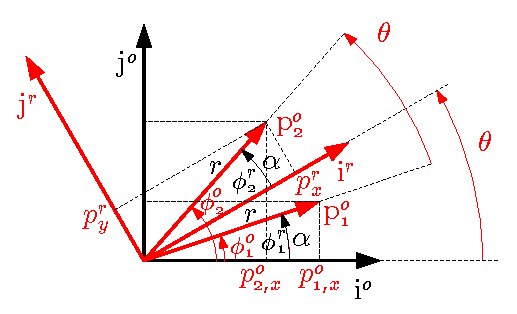
\includegraphics[scale=1.5]{figs/prueba.pdf} % Carga una figura llamada 
                                              % 'prueba.pdf' ubicada en
                                              % el folder 'figs'.
\end{center}
\vspace*{-1.0\baselineskip}     % Quita 1.0 líneas entre la figura y su 
                                % texto descriptivo. 
																
\caption{Ejemplo con una figura en formato PDF.} % Crea un texto 
                                                % descriptivo
                                                % para la figura.
\label{fig:ejemplo_figura_pdf}  % Agrega una etiqueta a la figura 
                                % para poder referenciarla.
\end{figure}
\end{Verbatim}

Un código similar al anterior permite generar las figuras~\ref{fig:ejemplo_figura_pdf},~\ref{fig:ejemplo_figura_jpg},~\ref{fig:ejemplo_figura_png}, las cuales se encuentran en formato PDF, JPG y PNG, respectivamente. Observe que la mejor figura es la figura~\ref{fig:ejemplo_figura_pdf} em formato PDF por sus nitidez y escalabilidad dado que está en formato vectorial.  Las figuras~\ref{fig:ejemplo_figura_jpg}, y \ref{fig:ejemplo_figura_png} se encuentran en formato raster y se {\em pixelean}.  No son escalables, por lo que debe evitar usar estos formatos salvo cuando incluirá una foto.  Para crear figuras en formato PDF puede utilizar Microsoft Visio$^\circledR$ de acuerdo a las instrucciones en el documento sobre como crear e incluir figuras.

Un ejemplo de como crear un espacio para agregar una figura posteriormente se muestra en la figura~\ref{fig:invisfig}.  Está figura vacía se construyó con el siguiente código.

\begin{Verbatim}[frame=single,framesep=5mm,rulecolor=\color{gray},numbers=left,numbersep=-10pt]
\begin{figure}[htbp]
\begin{center}
 %\includegraphics[scale=0.8]{}
 \fbox{\rule{10cm}{0cm}\rule{0cm}{6cm}}
\end{center}
\vspace*{-\baselineskip}
\caption{Un ejemplo de una figura vacía.}
\label{fig:invisfig} 
\end{figure}
\end{Verbatim}

\begin{figure}[htbp]
\begin{center}
 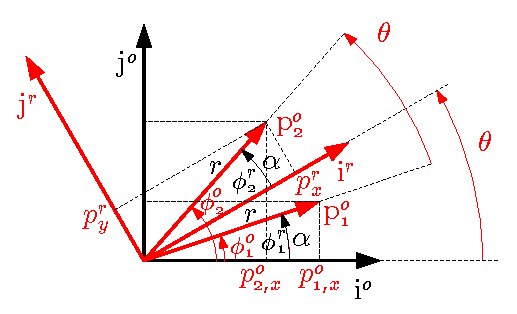
\includegraphics[scale=1.5]{figs/prueba.pdf}
\end{center}
\vspace*{-\baselineskip}
\caption{Ejemplo con una figura en formato PDF.}
\label{fig:ejemplo_figura_pdf} 
\end{figure}

\begin{figure}[htbp]
\begin{center}
 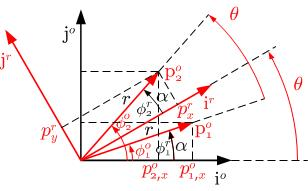
\includegraphics[scale=1.5]{figs/prueba.jpg}
\end{center}
\vspace*{-\baselineskip}
\caption{Ejemplo con una figura en formato JPG.}
\label{fig:ejemplo_figura_jpg} 
\end{figure}

\begin{figure}[htbp]
\begin{center}
 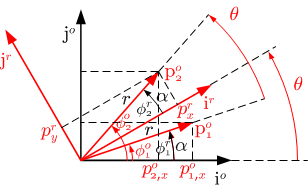
\includegraphics[scale=1.5]{figs/prueba.png}
\end{center}
\vspace*{-\baselineskip}
\caption{Ejemplo con una figura en formato PNG.}
\label{fig:ejemplo_figura_png} 
\end{figure}


\begin{figure}[htbp]
\begin{center}
 %\includegraphics[scale=0.8]{}
 \fbox{\rule{10cm}{0cm}\rule{0cm}{6cm}}
\end{center}
\vspace*{-\baselineskip}
\caption{Un ejemplo de una figura vacía.}
\label{fig:invisfig} 
\end{figure}


\section{Cómo incluir fórmulas y expresiones matemáticas}\label{sec:formulas}

Las fórmulas y expresiones matemáticas son parte del texto y siguen las mismas relgas de puntuación que una oración de texto tradicional.  Las fórmulas pueden incorporarse {\em en línea con el texto} o en forma {\em desplegada}.  En inglés se habla de {\em in-line equations} y {\em displayed equations}.

Ejemplos de expresiones matemáticas en línea se encuentran en las oraciones del siguiente párrafo.  

\begin{quote}
La fórmula de Euler establece que $e^{\imnum x} =\cos(x)+\imnum\sin(x)$.  La fórmula de De Moivre establece que $(\cos(x)+\imnum\sin(x))^n = (\cos(nx)+\imnum\sin(nx))^n$.  La fórmula de De Moivre se desprende fácilmente de la fórmula de Euler dado que $(\cos(nx)+\imnum\sin(nx))^n=(e^{\imnum x})^n=e^{\imnum nx}$. La fórmula de Euler a su vez puede demostrarse empleando la serie de potencias de la función exponencial $e^x$, y las expansiones de Taylor de $\cos(x)$ y $\sin(x)$.  La expansión en series de potencias de $e^z$ está dada por $e^z = 1 + \frac{z}{1!} + \frac{z^2}{2!} + \frac{z^3}{3!} + \cdots = \sum_{k=0}^\infty \frac{z^k}{k!}$.  La serie anterior evaluada en $z=\imnum x$ resulta después de reordenar los términos en 
$e^{ix} = \left ( 1 - \frac{x^2}{2!} + \frac{x^4}{4!} - \frac{x^6}{6!} + \frac{x^8}{8!} - \ldots \right )
        + \imnum \left ( x - \frac{x^3}{3!} + \frac{x^5}{5!} - \frac{x^7}{7!} + \ldots \right )$, donde las series entre paréntesis corresponden respectivamente a las series de Maclaurin de las funciones $\cos(x)$ y $\sin(x)$.
\end{quote}

En el párrafo anterior, las expresiones grandes son díficiles de leer porque se encuentran apretadas por el texto en las líneas anteriores y posteriores a las expresiones.  Para evitar este problema es que se utilizan ecuaciones desplegadas como se muestra en el siguiente párrafo.

\begin{quote}
La fórmula de Euler establece que $e^{\imnum x} =\cos(x)+\imnum\sin(x)$.  La fórmula de De Moivre establece que $(\cos(x)+\imnum\sin(x))^n = (\cos(nx)+\imnum\sin(nx))^n$.  La fórmula de De Moivre se desprende fácilmente de la fórmula de Euler dado que
$$ (\cos(nx)+\imnum\sin(nx))^n=(e^{\imnum x})^n=e^{\imnum nx}.$$

La fórmula de Euler a su vez puede demostrarse empleando la serie de potencias de la función exponencial $e^x$, y las expansiones de Taylor de $\cos(x)$ y $\sin(x)$.  La expansión en series de potencias de $e^z$ está dada por 
$$e^z = 1 + \frac{z}{1!} + \frac{z^2}{2!} + \frac{z^3}{3!} + \cdots = \sum_{k=0}^\infty \frac{z^k}{k!}.$$  La serie anterior evaluada en $z=\imnum x$ resulta después de reordenar los términos en 
$$e^{ix} = \left ( 1 - \frac{x^2}{2!} + \frac{x^4}{4!} - \frac{x^6}{6!} + \frac{x^8}{8!} - \ldots \right )
        + \imnum \left ( x - \frac{x^3}{3!} + \frac{x^5}{5!} - \frac{x^7}{7!} + \ldots \right ),$$ 
donde las series entre paréntesis corresponden respectivamente a las series de Maclaurin de las funciones $\cos(x)$ y $\sin(x)$.
\end{quote}

\begin{tipbox}{}
\begin{enumerate}
\item Es importante notar que en el ejemplo anterior, las expresiones grandes no solamente son más fáciles de leer porque aparecen desplegadas en una línea propia, sino que el uso puntuación es esencialemente la  misma que en el párrafo con ecuaciones en línea.  En resumen, al escribir ecuaciones desplegadas debe usar la misma puntuación que utilizarías al escribir una oración cualquiera considerando que las ecuaciones deben tratarse como si fuesen palabras regulares.

\item Para insterar ecuaciones o expresiones matemáticas {\em en línea} se encierra la expresión entre \$.
\vspace*{-\baselineskip}
\begin{center}
\begin{tabular}{|p{65mm}|p{65mm}|}
\hline
\parbox[t]{6cm}{
La fórmula de De Moivre se desprende fácilmente de la fórmula de Euler dado que
$(\cos(nx)+\imnum\sin(nx))^n=\left (e^{\imnum x}\right )^n=e^{\imnum nx}$.}
& \vspace*{-.5\baselineskip}
\begin{minipage}{7cm}
\begin{Verbatim}
La fórmula de De Moivre se 
desprende fácilmente de la 
fórmula de Euler dado que
$(\cos(nx)+\imnum\sin(nx))^n =
 \left (e^{\imnum x}\right )^n =
 e^{\imnum nx}$.

\end{Verbatim}
\end{minipage}
\\
\hline
\end{tabular}
\end{center}

\item Para insterar ecuaciones o expresiones matemáticas {\em desplegadas} se encierra la expresión entre \$\$ o entre \textbackslash [ y \textbackslash ].
\vspace*{-\baselineskip}
\begin{center}
\begin{tabular}{|p{65mm}|p{65mm}|}
\hline
\parbox[t]{6cm}{
La fórmula de De Moivre se desprende fácilmente de la fórmula de Euler dado que
$$(\cos(nx)+\imnum\sin(nx))^n=\left (e^{\imnum x}\right )^n=e^{\imnum nx}.$$}
& \vspace*{-.5\baselineskip}
\begin{minipage}{7cm}
\begin{Verbatim}
La fórmula de De Moivre se 
desprende fácilmente de la 
fórmula de Euler dado que
$$(\cos(nx)+\imnum\sin(nx))^n =
 \left (e^{\imnum x}\right )^n=
 e^{\imnum nx}.$$

\end{Verbatim}
\end{minipage}
\\
\hline
\end{tabular}
\end{center}

\item Para insterar ecuaciones o expresiones matemáticas {\em desplegadas} numeradas es necesario utilizar el ambiente \texttt{eqnarray}.
\vspace*{-\baselineskip}
\begin{center}
\begin{tabular}{|p{65mm}|p{65mm}|}
\hline
\parbox[t]{6cm}{
La fórmula de De Moivre se desprende fácilmente de la fórmula de Euler dado que
{\small
\begin{eqnarray}
\hspace*{-1em}(\cos(nx)+\imnum\sin(nx))^n
        &=&\left (e^{\imnum x}\right )^n\\
        &=&e^{\imnum nx}.
\end{eqnarray}
}
}
& \vspace*{-.5\baselineskip}
\begin{minipage}{7cm}
\begin{Verbatim}
La fórmula de De Moivre se 
desprende fácilmente de la 
fórmula de Euler dado que
\begin{eqnarray}
(\cos(nx)+\imnum\sin(nx))^n
 &=&\left (e^{\imnum x}
    \right )^n\\
 &=&e^{\imnum nx}.
\end{eqnarray}

\end{Verbatim}
\end{minipage}
\\
\hline
\end{tabular}
\end{center}

\end{enumerate}

\end{tipbox}

\begin{tipbox}

\begin{enumerate}

\item[5.] Finalmente, si hay una ecuación que debido a su relevancia considera que debe ser destacada de manera especial, esto se puede lograr con un comando específicamente creado para esta plantilla llamaodo \verb|eqbox|.  Por ejemplo, una ecuación desplegada y resaltada como:
\begin{eqnarray}
\eqbox{x^2 = 2\int_a^b x dx}
\end{eqnarray}
La expresión anterior se logra con el código:
\begin{Verbatim}[frame=single,framesep=5mm,rulecolor=\color{gray},numbers=left,numbersep=-10pt]
\begin{eqnarray}
\eqbox{x^2 = 2\int_a^b x dx}
\end{eqnarray}
\end{Verbatim}

\end{enumerate}

\end{tipbox}


\section{Cómo incluir tablas o figuras en ambientes \texttt{tcolorbox}}\label{sec:tab_figs_tcolorbox}

En los siguientes ejemplos se muestra como incluir una tabla o un gráfico dentro de un ambiente tipo \texttt{tcolorbox} como las cajas de definición \texttt{defbox}, las cajas de ejemplo \texttt{exbox}, y las cajas de recomendación \texttt{tipbox}.  En los ejemplos siguientes se usarán cajas de definición \texttt{defbox}, pero la explicación es igualmente válida para los otros ambientes mencionados que se basan en las cajas construidas entorno a la caja \texttt{tcolorbox}.  

En un \texttt{tcolorbox} no es posible colocar un ambiente flotante \texttt{figure} o \texttt{table} a menos que inserta la tabla declarando la opción \texttt{[H]} para forzar un elemento flotante dentro de otro elemento flotante como un \texttt{tcolorbox}.  Para usar la opción \texttt{[H]} deberá haber incluido el paquete \texttt{float} (incluido por defecto en esta plantilla).  La tabla~\ref{tab:basica} es un ejemplo de una tabla básica sin escalamiento.  En cambio, la tabla~\ref{tab:basica_escalada} es un ejemplo de un tabla escalada mediante el comnado \texttt{resizebox} que es parte del paquete \texttt{graphicx} o \texttt{graphics}.

\begin{Verbatim}[frame=single,framesep=5mm,rulecolor=\color{gray},numbers=left,numbersep=-10pt]
\begin{center}
\begin{defbox}{Tablas en ambientes \texttt{tcolorbox}}
Una tabla es una ordenación de datos en casillas o celdas de filas y 
columnas como se muestra a continuación.  Esta ordenación es también 
denominada un {\em arreglo} de datos en la que cada fila representa 
una entrada y las columnas representan diversos datos específicos o 
variables asociados a cada entrada.

\begin{table}[H]
\centering
\caption{Estructura de tabla básica.}
\label{tab:basica}
\begin{tabular}{r|ccc}
\multicolumn{1}{r}{}
& \multicolumn{1}{c}{Columna 1}
& \multicolumn{1}{c}{Columna 2}
& \multicolumn{1}{c}{Columna 3} \\ \cline{2-4}
Fila 1 & Celda 1,1 & Celda 1,2 & Celda 1,3 \\
Fila 2 & Celda 2,1 & Celda 2,2 & Celda 2,3
\end{tabular}%
\end{table}

\begin{table}[H]
\centering
\caption{Estructura de tabla básica escalada.}
\label{tab:basica_escalada}
\resizebox{\columnwidth}{!}{%
\begin{tabular}{r|ccccccccc}
\multicolumn{1}{r}{}
& \multicolumn{1}{c}{Columna 1}
& \multicolumn{1}{c}{Columna 2}
& \multicolumn{1}{c}{Columna 3}
& \multicolumn{1}{c}{Columna 4}
& \multicolumn{1}{c}{Columna 5}
& \multicolumn{1}{c}{Columna 6}
& \multicolumn{1}{c}{Columna 4}
& \multicolumn{1}{c}{Columna 5}
& \multicolumn{1}{c}{Columna 6} \\ \cline{2-9}
Fila 1 & Celda 1,1 & Celda 1,2 & Celda 1,3 & Celda 1,4 & 
  Celda 1,5 & Celda 1,6 & Celda 1,7 & Celda 1,8 & Celda 1,9 \\
Fila 2 & Celda 2,1 & Celda 2,2 & Celda 1,3 & Celda 2,4 &
  Celda 2,5 & Celda 2,6 & Celda 2,7 & Celda 2,8 & Celda 2,9
\end{tabular}%
} % end resizebox
\end{table}

\end{defbox}
\end{center}
\end{Verbatim}


\begin{center}
\begin{defbox}{Tablas en ambientes \texttt{tcolorbox}}
Una tabla es una ordenación de datos en casillas o celdas de filas y columnas como se muestra a continuación.  Esta ordenación es también denominada un {\em arreglo} de datos en la que cada fila representa una entrada y las columnas representan diversos datos específicos o variables asociados a cada entrada.

\begin{table}[H]
\centering
\caption{Estructura de tabla básica.}
\label{tab:basica}
\begin{tabular}{r|ccc}
\multicolumn{1}{r}{}
& \multicolumn{1}{c}{Columna 1}
& \multicolumn{1}{c}{Columna 2}
& \multicolumn{1}{c}{Columna 3} \\ \cline{2-4}
Fila 1 & Celda 1,1 & Celda 1,2 & Celda 1,3 \\
Fila 2 & Celda 2,1 & Celda 2,2 & Celda 2,3
\end{tabular}%
\end{table}

\begin{table}[H]
\centering
\caption{Estructura de tabla básica escalada.}
\label{tab:basica_escalada}
\resizebox{\columnwidth}{!}{%
\begin{tabular}{r|ccccccccc}
\multicolumn{1}{r}{}
& \multicolumn{1}{c}{Columna 1}
& \multicolumn{1}{c}{Columna 2}
& \multicolumn{1}{c}{Columna 3}
& \multicolumn{1}{c}{Columna 4}
& \multicolumn{1}{c}{Columna 5}
& \multicolumn{1}{c}{Columna 6}
& \multicolumn{1}{c}{Columna 4}
& \multicolumn{1}{c}{Columna 5}
& \multicolumn{1}{c}{Columna 6} \\ \cline{2-9}
Fila 1 & Celda 1,1 & Celda 1,2 & Celda 1,3 & Celda 1,4 & Celda 1,5 & Celda 1,6 & Celda 1,7 & Celda 1,8 & Celda 1,9 \\
Fila 2 & Celda 2,1 & Celda 2,2 & Celda 1,3 & Celda 2,4 & Celda 2,5 & Celda 2,6 & Celda 2,7 & Celda 2,8 & Celda 2,9
\end{tabular}%
} % end resizebox
\end{table}

\end{defbox}
\end{center}

Incluir una figura en una caja de definición es igual que en el caso de las tablas.  Las figuras y tablas pueden incluirse directamente usando \texttt{includefigure} o \texttt{tabular} sin {\em rodear} estos objetos por sus ambientes \texttt{figure} o \texttt{table}.  Sin embargo, si uno quiere insertar una figura o tabla con su título enumerado en forma automática a través de \texttt{caption}, entonces será neceario añadir la opción \texttt{[H]} para forzar un elemento flotante. 

\begin{Verbatim}[frame=single,framesep=5mm,rulecolor=\color{gray},numbers=left,numbersep=-10pt]
\begin{center}
\begin{defbox}{Figuras en ambientes \texttt{tcolorbox}}
La primera es la figura incluida sin usar el ambiente flotante 
\texttt{figure}, por lo que no puede usarse el comando \texttt{caption} 
para ponerle un título enumerado automáticamente.  Sin embargo, es una 
manera rápida y simple de incluir una figura cuando no se requiere 
títulos adicionales.

\begin{center}
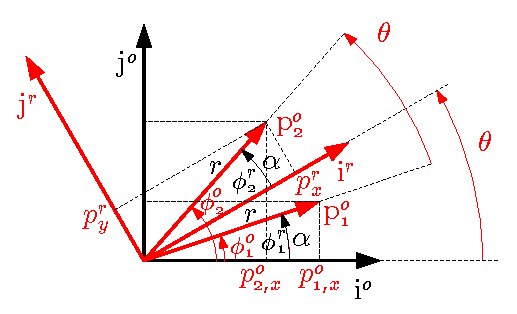
\includegraphics[scale=1.0]{figs/prueba.pdf}
\end{center}

La segunda es una figura incluida usando el ambiente flotante 
\texttt{figure}.

\begin{figure}[H]
\centering
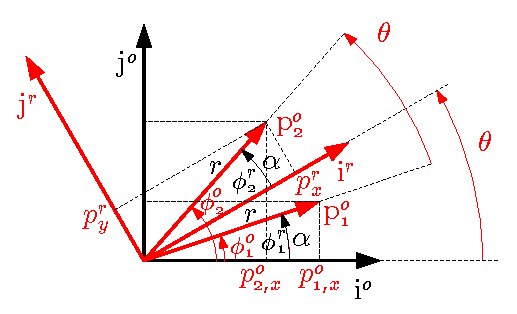
\includegraphics[scale=1.0]{figs/prueba.pdf}
\vspace*{-1.0\baselineskip}
\caption{Una figura dentro de una ambiente \texttt{tcolorbox}.}
\end{figure}

\end{defbox}
\end{center}
\end{Verbatim}

\begin{center}
\begin{defbox}{Figuras en ambientes \texttt{tcolorbox}}
La primera es la figura incluida sin usar el ambiente flotante \texttt{figure}, por lo que no puede usarse el comando \texttt{caption} para ponerle un título enumerado automáticamente.  Sin embargo, es una manera rápida y simple de incluir una figura cuando no se requiere títulos adicionales.

\begin{center}
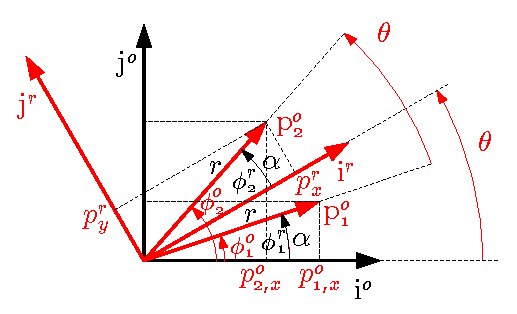
\includegraphics[scale=1.0]{figs/prueba.pdf}
\end{center}

La segunda es una figura incluida usando el ambiente flotante \texttt{figure}.

\begin{figure}[H]
\centering
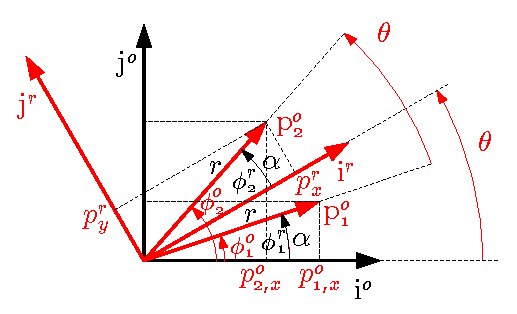
\includegraphics[scale=1.0]{figs/prueba.pdf}
\vspace*{-1.0\baselineskip}
\caption{Una figura dentro de una ambiente \texttt{tcolorbox}.}
\end{figure}

\end{defbox}
\end{center}


\section{Notación}\label{sec:notacion}

La notación a emplearse en los apuntes del curso debe ceñirse a la notación estándar de los textos de referencia y que se resume en:
\begin{itemize}
\item \url{https://en.wikipedia.org/wiki/List_of_mathematical_symbols_by_subject}
\item \url{https://en.wikipedia.org/wiki/List_of_mathematical_symbols} 
\end{itemize}

A continuación se resumen algunos símbolos y convenciones que debemos utilizar en nuestros apuntes.  Entre paréntesis se indica el comando \LaTeX que lo genera, así como el nombre resumido que se incluye en la plantilla \texttt{header.tex}.

% Create a new length to control the width of the definition column in
% the "notation table", to be used with parbox.
\newlength{\hdiml} % left  column width
\newlength{\hdim}  % right column width
\newlength{\lsk}   % line skip
%\settowidth{\hdim}{\hspace{\textwidth}\hspace{-3cm}}
\settowidth{\hdiml}{\hspace{.2\textwidth}}
\settowidth{\hdim }{\hspace{.8\textwidth}}
\setlength{\lsk  }{1.3ex}

\subsection{Definiciones Generales Fundamentales}

{\bf Sintáxis General}
\begin{tabbing}
\hspace{\hdiml} \= \hspace{\hdim} \kill
$\eqbydef $    \> Denotes definition.\\[\lsk] %formerly  :=
$|$            \> Denota ``tal que''.\\[\lsk]
i.e.           \> Significa ``es decir'' (en latín {\em id est}).\\[\lsk]
e.g.           \> Significa ``por ejemplo'' (en latín {\em exempli gratia}).\\[\lsk]
q.e.d.         \> \parbox[t]{\hdim}{Significa ``queda esto demostrado'' e indica el fin de una demostración.  En latín ``quod erat demonstrandum'' significa literalemente ``como debíase demostrar''.}\\[\lsk]
\end{tabbing}

{\bf Constantes y Símbolos Matemáticos}
\begin{tabbing}
\hspace{\hdiml} \= \hspace{\hdim} \kill
$\pi$    \> La constante de Arquímedes $\pi=3.1415926...$.\\[\lsk]
$e$    \> La constante de Euler $e=2.7182818...$.\\[\lsk]
$\imnum$    \> El número imaginario $\sqrt{-1}$.\\[\lsk]
$\varphi$   \> La razón áurea $\phi =  (1+\sqrt{5})/2 = 1.6180339...$.\\[\lsk]
$\infty$ \> Infinito.\\[\lsk]
\end{tabbing}


\subsection{Teoría de Conjuntos}

{\bf Construcción de Conjuntos}
\begin{tabbing}
\hspace{\hdiml} \= \hspace{\hdim} \kill
$\emptyset$    \> Conjunto vacío. (\Verb|\emptyset|)\\[\lsk]
$\{a,b,\ldots\}$ \> Conjunto de elementos $a$, $b$, etc.  (\Verb|\{a,b,\ldots\}|)\\[\lsk]
$\{x:T(x)\}$ \> \parbox[t]{\hdim}{Construcción de conjuntos de elementos $x$ que satisfacen 
                  la condición $T(x)$. % (\Verb|\{x:T(x)\}|)
									}\\[\lsk]
\end{tabbing}


{\bf Operaciones con Conjuntos}
\begin{tabbing}
\hspace{\hdiml} \= \hspace{\hdim} \kill
$A\cup B$         \> Unión de conjuntos $A$ y $B$.\\[\lsk]
$A\cap B$         \> Intersección de conjuntos $A$ y $B$.\\[\lsk]
$A^C$         \> Complemento del conjungo $A$.\\[\lsk]
$A^\circ$      \> Interior del conjunto $A$.\\[\lsk]
$\bar{A}$      \> Cierre del conjunto $A$.\\[\lsk]
$\flat(A)$     \> Borde del conjunto $A$.\\[\lsk]
$A\setminus B$ \> \parbox[t]{\hdim}{Resta de conjuntos $A$ menos $B$, i.e. conjunto $A$ excluyendo aquellos elementos que pertenencen al conjunto $B$.}\\[\lsk]
\end{tabbing}

{\bf Relaciones entre Conjuntos}
\begin{tabbing}
\hspace{\hdiml} \= \hspace{\hdim} \kill
$A\subset B$         \> $A$ es un subconjunto propio de $B$.\\[\lsk]
$A\subseteq B$       \> $A$ es un subconjunto de $B$.\\[\lsk]
$A\supset B$         \> $A$ es un supraconjunto propio de $B$.\\[\lsk]
$A\supseteq B$       \> $A$ es un supraconjunto de $B$.\\[\lsk]
$a\in A$       \> El elemento $a$ pertenence al conjunto $A$.\\[\lsk]
$A\ni a$       \> El conjunto $A$ posee un elemento $a$.\\[\lsk]
$a\notin A$       \> El elemento $a$ no pertenence al conjunto $A$.\\[\lsk]
$A\not\ni a$       \> El conjunto $A$ no posee un elemento $a$.\\[\lsk]
\end{tabbing}


{\bf Conjuntos de Números}
\begin{tabbing}
\hspace{\hdiml} \= \hspace{\hdim} \kill
$\natnums$  \> Conjunto de números enteros estrictamente positivos 
               $\{1,2,3,\ldots\}$.\\[\lsk] %CH2
$\intnums$  \> % Ring
Conjunto de números enteros $\{\ldots,-2,-1,0,1,2,\ldots\}$.\\[\lsk]
$\intnums_+$\> Conjunto de enteros no-negativos $\{0,1,2,\ldots\}$, 
               note que $\intnums_+\equiv \natnums\cup\{0\}$.\\[\lsk] %CH2
$\mathbb{Q}$\> Conjunto de los números racionales.\\[\lsk]
$\reals$    \> % Field 
               Conjunto de los números reales.\\[\lsk] %CH2
$\reals_+$, ($\reals_-$) \> Conjunto de los reales non-negativos $[0,\infty)$  
                            (no-positivos $(-\infty,0]$).\\[\lsk] %CH2
$\reals^n$  \> Espacio Euclideano  $n$-dimensional.\\[\lsk] %CH2
$\complex$  \> % Field 
               Conjunto de los números complejos, $\complex = \{s=a+\imnum b\ |\ a\in\reals, b\in\reals\}$.\\[\lsk]
$\complex_+$, ($\complex_-$) \> 
             \parbox[t]{\hdim}{
             Conjunto de los números complejos en el semi-plano derecho (izquierdo),
             incluyendo el eje imaginario, i.e. 
           $\complex_+\eqbydef \{a+\imnum b\in\complex~|~a\in\reals_+, b\in\reals\}$, 
           (respectivamente, $\complex_-\eqbydef \{a+\imnum b\in\complex~|~a\in\reals_-, b\in\reals\}$).
						}\\[\lsk] %CH5
$\complex_+^\circ$, ($\complex_-^\circ$) \>
           \parbox[t]{\hdim}{
           Interior de $\complex_+$, i.e. 
           $\complex_+^\circ\eqbydef \{a+\imnum b\in\complex~|~a,b\in\reals, a>0 \}$, 
           (respectivamente, el interior de $\complex_-$, i.e. $\complex_-^\circ\eqbydef \{a+\imnum b\in\complex~|~a,b\in\reals, a<0 \}$).}\\[\lsk] %CH5

\end{tabbing}

{\bf Cardinalidad}
\begin{tabbing}
\hspace{\hdiml} \= \hspace{\hdim} \kill
$|A|$ o $\#A$  \> Cardinalidad del conjunto $A$.\\[\lsk]
\end{tabbing}


\subsection{Aritmética}

{\bf Operadores Aritméticos}
\begin{tabbing}
\hspace{\hdiml} \= \hspace{\hdim} \kill
$a+b$  \> Adición de $a$ y $b$.\\[\lsk]
$a-b$  \> Sustracción de $b$ a $a$.\\[\lsk]
$a\cdot b$ \> Multiplicación de $a$ y $b$.\\[\lsk]
$a/b$, $a\div b$, $\frac{a}{b}$ \> División de $a$ por $b$.\\[\lsk]
$-a$   \> Negativo del número $a$.\\[\lsk]
$\pm a$, $\mp a$ \> Más o menos $a$, menos o más $a$.\\[\lsk]
$(expr)$, $[expr]$ \> La expresión $expr$ entre parétesis debe ser evaluada primero.\\[\lsk] 
\end{tabbing}

{\bf Signos de Igualdad}
\begin{tabbing}
\hspace{\hdiml} \= \hspace{\hdim} \kill
$a=b$  \> $a$ es igual a $b$.\\[\lsk]
$a\neq b$  \> $a$ es distinto de $b$.\\[\lsk]
$a\equiv b$ \> $a$ es idéntico a $b$.\\[\lsk]
$a\approx b$ \> $a$ es aproximadamente igual a $b$.\\[\lsk]
$a\sim b$ \> $a$ es proporcional a $b$.\\[\lsk]
$a\propto b$ \> $a$ es proporcional a $b$.\\[\lsk]
\end{tabbing}

{\bf Comparación}
\begin{tabbing}
\hspace{\hdiml} \= \hspace{\hdim} \kill
$a<b$  \> $a$ es menor a $b$.\\[\lsk]
$a>b$  \> $a$ es mayor a $b$.\\[\lsk]
$a\leq b$ \> $a$ es menor o igual a $b$.\\[\lsk]
$a\geq b$ \> $a$ es mayor o igual a $b$.\\[\lsk]
$a\ll b$ \> $a$ es mucho menor a $b$.\\[\lsk]
$a\gg b$ \> $a$ es mucho mayor a $b$.\\[\lsk]
\end{tabbing}

{\bf Intervalos}
\begin{tabbing}
\hspace{\hdiml} \= \hspace{\hdim} \kill
$[a,b]$  \> Intervalo cerrado entre $a$ y $b$.\\[\lsk]
$(a,b)$  \> Intervalo abierto entre $a$ y $b$.\\[\lsk]
$[a,b)$ \> Intervalo entre $a$ y $b$, que incluye a $a$, pero no incluye a $b$.\\[\lsk]
$(a,b]$ \> Intervalo entre $a$ y $b$, que no incluye a $a$, pero incluye a $b$.\\[\lsk]
\end{tabbing}


\newpage6
{\bf Aritmética Básica de Números Complejos}
\begin{tabbing}
\hspace{\hdiml} \= \hspace{\hdim} \kill
$\mbox{Re}(s)$ \> Parte real del complejo $s$.  Si $s=a+\imnum b$, entonces $\mbox{Re}(s)=a$.\\[\lsk]
$\mbox{Im}(s)$ \> Parte imaginaria del complejo $s$.  Si $s=a+\imnum b$, entonces $\mbox{Im}(s)=b$.\\[\lsk]
$s^*$ \> Complejo $s$ conjugado.  Si $s=a+\imnum b$, entonces $s^*=a-\imnum b$.\\[\lsk]
$|s|$ \> Magnitud del complejo $s$.  Si $s=a+\imnum b$, entonces $|s|=\sqrt{a^2+b^2}$.\\[\lsk]
$\angle s$ \> Angulo del complejo $s$.  Si $s=a+\imnum b$, entonces $\angle s=\arctan(b/a)$.\\[\lsk]
\end{tabbing}


\subsection{Cálculo}

{\bf Secuencias y series}
\begin{tabbing}
\hspace{\hdiml} \= \hspace{\hdim} \kill
$\sum_{i=1}^n a_i$ \> \parbox[t]{\hdim}{Sumatoria de los elementos $a_i$ desde $i=1$ hasta $i=n$, es decir $a_1+a_2+\cdots+a_{n-1}+a_n$.}\\[\lsk]
$\sum_{i\in I} a_i$ \> Sumatoria de los elementos $a_i$ tales que $i\in I$.\\[\lsk]
$\prod_{i=1}^n a_i$ \> \parbox[t]{\hdim}{Multiplicatoria de los elementos $a_i$ desde $i=1$ hasta $i=n$, es decir $a_1\cdot a_2\cdot \ldots \cdot a_{n-1}\cdot a_n$.}\\[\lsk]
$\prod_{i\in I} a_i$ \> Multiplicatoria de los elementos $a_i$ tales que $i\in I$.\\[\lsk]
$(a_n)$ \> Secuencia de elementos $a_0, a_1, a_2, \ldots$.\\[\lsk]
$a_n\rightarrow a$ \> La secuencia $a_n$ tiende a $a$.\\[\lsk]
\end{tabbing}

{\bf Funciones}
\begin{tabbing}
\hspace{\hdiml} \= \hspace{\hdim} \kill
$f:A\rightarrow B$ \> \parbox[t]{\hdim}{La función $f$ mapea el conjunto $A$ al conjunto $B$.}\\[\lsk]
$f:x\mapsto y$ \> \parbox[t]{\hdim}{La función $f$ mapea el elemento $x$ al elemento $y$.}\\[\lsk]
$f(x)$ \> Imagen del elemento $x$ bajo la función $f$.\\[\lsk]
$f(\cdot)$ \> \parbox[t]{\hdim}{El argumento $\cdot$ de la función $f$ es un comodín que debe ser reemplazado por algo posteriormente.}\\[\lsk]
$f^{-1}$ \> \parbox[t]{\hdim}{Es la función inversa de $f$.}\\[\lsk]
$f\circ g$ \> \parbox[t]{\hdim}{Composición de las funciones $f$ y $g$.}\\[\lsk]
\end{tabbing}


\newpage
\subsection{Algebra Lineal y Geometría}

{\bf Geometría Elemental}
\begin{tabbing}
\hspace{\hdiml} \= \hspace{\hdim} \kill
$\overline{AB}$ \> \parbox[t]{\hdim}{Segmento entre los puntos $A$ y $B$.}\\[\lsk]
$\overline{AB}$ \> \parbox[t]{\hdim}{Largo del segmento entre los puntos $A$ y $B$.}\\[\lsk]
$\vec{AB}$ \> \parbox[t]{\hdim}{Vector entre los puntos $A$ y $B$.}\\[\lsk]
$\angle{ABC}$ \> \parbox[t]{\hdim}{Angulo entre los segmentos $BA$ y $BC$.}\\[\lsk]
$\triangle{ABC}$ \> \parbox[t]{\hdim}{Triángulo con vértices $A$, $B$ y $C$.}\\[\lsk]
$\square{ABCD}$ \> \parbox[t]{\hdim}{Cuadrilátero con vértices $A$, $B$, $C$ y $D$.}\\[\lsk]
$\ell_1\parallel\ell_2$ \> \parbox[t]{\hdim}{Líneas $\ell_1$ y $\ell_2$ son paralelas.}\\[\lsk]
$\ell_1\nparallel\ell_2$ \> \parbox[t]{\hdim}{Líneas $\ell_1$ y $\ell_2$ no son paralelas.}\\[\lsk]
$\ell_1\perp\ell_2$ \> \parbox[t]{\hdim}{Líneas $\ell_1$ y $\ell_2$ son perpendiculares.}\\[\lsk]
\end{tabbing}

{\bf Vectores y Matrices}
\begin{tabbing}
\hspace{\hdiml} \= \hspace{\hdim} \kill
$[v_1\ v_2\ \cdots\ v_n]$ \> \parbox[t]{\hdim}{Vector fila de elementos $v_1, v_2,\ldots, v_n$.}\\[\lsk]
$\left [
\begin{array}{c}v_1\\ v_2\\ \vdots\\ v_n\end{array}
\right ]$ \> \parbox[t]{\hdim}{Vector columna de elementos $v_1, v_2,\ldots, v_n$.}\\[\lsk]
$\left [
\begin{array}{cccc}
a_{11}&a_{12}&\cdots&a_{1n}\\ 
a_{21}&a_{22}&\cdots&a_{2n}\\
\vdots&\vdots&\ddots&\vdots\\
a_{m1}&a_{m2}&\cdots&a_{mn}
\end{array}
\right ]$
 \> \parbox[t]{\hdim}{\vspace*{-\baselineskip}\hspace*{3em} Matriz de elementos $a_{ij}$ en la fila $i$ y columna $j$,\\ 
                      \hspace*{3em} de $m$ filas y $n$ columnas.}\\[\lsk]
\end{tabbing}

{\bf Cálculo Vectorial}
\begin{tabbing}
\hspace{\hdiml} \= \hspace{\hdim} \kill
$\mathbf{v}\cdot \mathbf{w}$ \> \parbox[t]{\hdim}{Producto punto entre los vectores $\mathbf{v}$ y $\mathbf{w}$.}\\[\lsk]
$\mathbf{v}\times \mathbf{w}$ \> \parbox[t]{\hdim}{Producto cruz entre los vectores $\mathbf{v}$ y $\mathbf{w}$.}\\[\lsk]
$\mathbf{v}^T$         \> La letra $T$ superscrita denota {\em transposición} del vector $\mathbf{v}$.\\[\lsk]
$\|\mathbf{v}\|$ \> \parbox[t]{\hdim}{Norma del vector $\mathbf{v}$.}\\[\lsk]
$\hat{\mathbf{v}}$ \> \parbox[t]{\hdim}{Vector $\mathbf{v}$ normalizado.}\\[\lsk]
\end{tabbing}

\newpage
{\bf Cálculo Matricial}
\begin{tabbing}
\hspace{\hdiml} \= \hspace{\hdim} \kill
$\mathbf{A}\cdot \mathbf{B}$ \> \parbox[t]{\hdim}{Producto de las matrices $\mathbf{A}$ y $\mathbf{B}$.}\\[\lsk]
$\mathbf{A}^T$         \> La letra $T$ superscrita denota {\em transposición} de la matriz $\mathbf{A}$.\\[\lsk]
$\mathbf{A}^{-1}$         \> Inversa de la matriz $\mathbf{A}$.\\[\lsk]
$|\mathbf{A}|$ \> \parbox[t]{\hdim}{Determinante de la matriz $\mathbf{A}$.}\\[\lsk]
$\|\mathbf{A}\|$ \> \parbox[t]{\hdim}{Norma de la matriz $\mathbf{A}$.}\\[\lsk]

\end{tabbing}


\subsection{Combinatórica}

{\bf Combinatórica Elemental}
\begin{tabbing}
\hspace{\hdiml} \= \hspace{\hdim} \kill
$n!$ \> \parbox[t]{\hdim}{Factorial de $n$, $n!=n\cdot (n-1)\cdot (n-2)\cdots 2\cdot 1$.}\\[\lsk]
$\binom{n}{k}$ \> \parbox[t]{\hdim}{Coeficiente binomial $k$ de $n$, es el número de combinaciones de $k$ elementos elegidos de un total de $n$ elementos sin  repetición.}\\[\lsk]
\end{tabbing}


\subsection{Probabilidades y Estadística}

{\bf Probabilidades y Estadística Elementales}
\begin{tabbing}
\hspace{\hdiml} \= \hspace{\hdim} \kill
$P(A)$ \> \parbox[t]{\hdim}{Probabilidad del evento $A$.}\\[\lsk]
$P(A|B)$ \> \parbox[t]{\hdim}{Probabilidad condicional del evento $A$ dado el evento $B$.}\\[\lsk]
$E(X)$ \> \parbox[t]{\hdim}{Valor esperado de la variable aleatoria $X$.}\\[\lsk]
$V(X)$ \> \parbox[t]{\hdim}{Varianza de la variable aleatoria $X$.}\\[\lsk]
$\mu(X)$ \> \parbox[t]{\hdim}{Media de la variable aleatoria $X$.}\\[\lsk]
$\sigma(X)$ \> \parbox[t]{\hdim}{Desviación estándar de la variable aleatoria $X$.}\\[\lsk]
$\sigma^2(X)$ \> \parbox[t]{\hdim}{Varianza de la variable aleatoria $X$.}\\[\lsk]
$\sigma(X,Y)$ \> \parbox[t]{\hdim}{Covarianza de las variables aleatorias $X$ e $Y$.}\\[\lsk]
$\rho(X,Y)$ \> \parbox[t]{\hdim}{Correlación de las variables aleatorias $X$ e $Y$.}\\[\lsk]
$X\sim F)$ \> \parbox[t]{\hdim}{La variable aleatoria $X$ tiene distribución $F$.}\\[\lsk]
$X\approx F)$ \> \parbox[t]{\hdim}{La variable aleatoria $X$ tiene distribución aproximadamente $F$.}\\[\lsk]
$\overline{x}$ \> \parbox[t]{\hdim}{Promedio de los valores $x_1,x_2,\ldots,x_n$.}\\[\lsk]
\end{tabbing}


\subsection{Lógica}

{\bf Operadores}
\begin{tabbing}
\hspace{\hdiml} \= \hspace{\hdim} \kill
$A\wedge B$ \> \parbox[t]{\hdim}{Proposición $A$ y proposición $B$.}\\[\lsk]
$A\vee B$ \> \parbox[t]{\hdim}{Proposición $A$ o proposición $B$, o ambas.}\\[\lsk]
$A\oplus B$ \> \parbox[t]{\hdim}{Ya sea la proposición $A$ o la proposición $B$, pero no ambas. Este operador es el llamado ``o exclusivo''.}\\[\lsk]
$\sim A$, $\overline{A}$, $\lnot A$ \> \parbox[t]{\hdim}{La proposición $A$ negada (``no $A$'').}\\[\lsk]
$A\Rightarrow B$ \> \parbox[t]{\hdim}{La proposición $A$ implica de $B$.}\\[\lsk]
$A\Leftrightarrow B$ \> \parbox[t]{\hdim}{La proposición $A$ implica $B$ y viceversa.}\\[\lsk]
\end{tabbing}

{\bf Cuantificadores}
\begin{tabbing}
\hspace{\hdiml} \= \hspace{\hdim} \kill
$\forall x$ \> \parbox[t]{\hdim}{Para todo $x$.}\\[\lsk]
$\exists x$ \> \parbox[t]{\hdim}{Existe al menos un elemento $x$.}\\[\lsk]
$\exists! x$ \> \parbox[t]{\hdim}{Existe exactamente un elemento $x$.}\\[\lsk]
$\nexists x$ \> \parbox[t]{\hdim}{No existe un elemento $x$.}\\[\lsk]
\end{tabbing}

{\bf Símbolos de Deducción}
\begin{tabbing}
\hspace{\hdiml} \= \hspace{\hdim} \kill
$\Rightarrow\Leftarrow$ \> \parbox[t]{\hdim}{Contradicción.}\\[\lsk]
$A\therefore B$ \> \parbox[t]{\hdim}{La proposición $A$ es verdadera, por lo tanto $B$ es verdadera.}\\[\lsk]
$A\because B$ \> \parbox[t]{\hdim}{La proposición $A$ es verdadera, porque $B$ es verdadera.}\\[\lsk]
$\blacksquare$, $\square$ \> \parbox[t]{\hdim}{q.e.d. (fin de la demostración).}\\[\lsk]
\end{tabbing}



\begin{enumerate}
\setcounter{enumi}{\value{total}}
\item Q1: \bu{This is bold underlined text.}
\item Q2
\item Q3

\setcounter{total}{\value{enumi}}
\end{enumerate}



\newpage
\section{Algunas cosas de la plantilla antigua...}

En las siguientes subsecciones se muestra principalmente por motivos históricos varias cosas que formaban parte de la plantilla antigua.  En principio nada de lo que está en esta sección debiese ser utilizado en las versiones finales de los apuntes.  Sin embargo, hay algunos trucos que pueden ser interesantes, commo el ejemplo de cómo hacer listas enumeradas que parten con la numeración de la lista anterior, y cómo hacer una plantilla de manual.

\subsection{Ejemplo de listas enumeradas que parten con la numeración de la lista anterior}

\subsubsection{Una primera lista enumerada}\label{sec:primera_lista}
\setcounter{total}{0}
\begin{enumerate}
\setcounter{enumi}{\value{total}}
% Esta frase era antes de otra.
\item Q1 Vea la sección \ref{sec:segunda lista}. La variable $x$ sumada a la $y$ resulta en $x+y$.
\item Q2
\item Q3

\setcounter{total}{\value{enumi}}
\end{enumerate}

\subsubsection{Una segunda lista enumerada continuando desde la anterior}\label{sec:segunda_lista}
\begin{enumerate}
\setcounter{enumi}{\value{total}}
\item Q4
\item Q5
\item Q6

\setcounter{total}{\value{enumi}}
\end{enumerate}

\subsection{Algunos Ejemplos Enmarcados con Recuadros}
Estos Ejemplos con  Recuadros {\em Boxed Examples} siguen el formato empleado en la plantilla antigua.  No use esta manera de hacer recuadros en los documentos nuevos.  Para hacer ejemplos enmarcados en recuadros, por favor utilice las indicaciones presentadas en la sección~\ref{sec:ejemplo}.

\begin{example}
$X \equiv$ toss a coin ($\leftarrow$ this is the {\em process}).\\[1ex]
$x_0 = \textrm{head}$\\[1ex]
$x_1 = \textrm{tail}$\\[1ex]
\end{example}

\begin{example}
$X \equiv$ draw some number of candies with a spoon.\\[1ex]
$P(X=x_i) = \frac{n_i}{N}$ where $n_i$ is the number of times the amount $x_i$  was drawn, $i=1,2,\ldots I$.\\[1ex]
\end{example}

\subsection{Algunas Definiciones Enmarcadas con Recuadros}
Estas Definciones Emarcadas {\em Boxed Definitionss} siguen el formato empleado en la plantilla antigua.  No use esta manera de hacer recuadros en los documentos nuevos.  Para hacer definiciones enmarcadas en recuadros, por favor utilice las indicaciones presentadas en la sección~\ref{sec:definicion}.


\defboxB[Probability Law]{
\begin{eqnarray}
\sum_{i=1}^{\infty} P(x_i) = 1,\hspace{4em}\int_{-\infty}^{\infty} p(x)dx = 1
\end{eqnarray}
}

\defboxB[\parbox{0.8\textwidth}{Probabilidades no-condicionadas individuales\\{\em (}unconditional individual probabilities{\em )}}]{
\begin{eqnarray}
P(x_i)&=&\frac{{n_X}_i}{N},\hspace{4em} i=1,\ldots,I\\
P(y_j)&=&\frac{{n_Y}_j}{N},\hspace{4em} j=1,\ldots,I
\end{eqnarray}
}

\defboxB{Something in the air.}


\chapter*{\vspace*{-2\baselineskip}Appendix: Robot Design and Engineering}\addcontentsline{toc}{chapter}{Appendix: Robot Design and Engineering}

Este es un ejemplo de como incluir un apéndice y la estructura estándar de un manual de software.
\section{General Background}

\section{Procedure}

\section{Function Reference}
\frefex

\subsection{recfunc}\label{ss:recfunc}
\begin{fref}
%\fpurp{something}
\bfverbatim{Examples}
Consider the Zetino basis, \verb|Z|, given in the example for the
function \verb|zfunction| on page~\pageref{ss:zfunction}.  
Additionally, suppose that $Z_6=[f_1,f_2]=0$, then the Zetino algebra 
can be expressed in terms of the following 3-dimensional basis of 
independent Zetino products, in terms of which \verb|z4| is expressed 
(see the example for the function \verb|zfunction| on 
page~\pageref{ss:zfunction}): 
\begin{verbatim}
  Z := [f0~, f1~, f0~ *f1~, f0~*(f0~ *f1~),
         f1~*(f0~*(f0~*f1~))]
\end{verbatim}
\efverbatim
\bfverbatim{Salut!}
Carambola
\begin{verbatim}
Is the problem of creating something literally #@?&$!* stupid!
\end{verbatim}
\efverbatim
\bfverbatim{}
Alobmarac
\begin{verbatim}
Is the problem of inverting something totally silly!
\end{verbatim}
\efverbatim
\end{fref}


\begin{fref}%
\fpurp{Calcular Pitagoras.}%
\fsynt{\texttt{c(a,b)}}%
\fdesc{This function computes something using the $\alpha(X)$ algorithm.%
\begin{eqnarray}%
c(a,b) = a^2 + b^2%
\end{eqnarray}%
}%
\fargs{$v_1$\hspace{1cm}\=The value of the first argument.\\%
\>$v_2$\>The value of the second argument.\\%
\>$\vdots$\>\\%
\>$v_n$\>The value of the $n$-th argument.%
}%
\end{fref}

\end{document}